% !TEX root = main.tex
\section{Service Discovery}\label{sec:results}
In this section, we provide a comprehensive overview of services on anycast, focusing on the most relevant and interesting ones.
We show the correlation of services and network operators, and how services are replicated. 
Finally, we analyze the differences in accessing a service from different \glspl{vp}. 
We detect and group the responsiveness of anycast prefixes in our \dataset according to Sattler \etal~\cite{SattlerEtAl_PackedBrimInvestigating_2023}.
The results we present are based on the merged measurements of February 18th and 20th (pipeline) from one \gls{vp} in Europe. 
We mention when additional data from other campaigns is used.

\subsection{Transport Layer}\label{subsec:transport_layer}
\begin{table}[tb]
\centering
%\small
\caption{Transport protocols (filtered post-HRP classification). Columns show \textit{active IPs},  /24-prefix with \textit{active IPs}, and ASes with at least one prefix with detected service.}
\label{tab:transport_protocols}
\begin{tabular}{l r@{~}l r@{~}l r@{~}l}
\toprule
 & \multicolumn{2}{c}{Services (IP)} & \multicolumn{2}{c}{Services (/24)} & \multicolumn{2}{c}{Services (ASes)} \\
\midrule
HRP & \multicolumn{2}{c}{\num{1.6e6}} & \multicolumn{2}{c}{\num{9.4e3}} & \multicolumn{2}{c}{\num{177}} \\
\midrule
TCP & \num{895.2e3} & (55\%) & \num{9.2e3} & (98\%) & \num{153} & (86\%) \\
UDP & \num{65.4e3} & (4\%) & \num{591} & (6\%) & \num{65} & (37\%) \\
QUIC & \num{1.1e6} & (66\%) & \num{4.9e3} & (53\%) & \num{89} & (51\%) \\
\midrule
Non-HRP & \multicolumn{2}{c}{\num{141.9e3}} & \multicolumn{2}{c}{\num{3.8e3}} & \multicolumn{2}{c}{\num{823}} \\
\midrule
TCP & \num{113e3} & (80\%) & \num{2.4e3} & (63\%) & \num{535} & (65\%) \\
UDP & \num{30.9e3} & (22\%) & \num{2.4e3} & (64\%) & \num{646} & (78\%) \\
QUIC & \num{3.5e3} & (2\%) & \num{651} & (17\%) & \num{93} & (11\%) \\
\bottomrule
\end{tabular}
\vspace*{-4mm}
\end{table}

We see that for 96\% of all /24 anycast prefixes, at least one IP address hosts at least one service.
Overall, \glspl{hrp} and non-\glspl{hrp} exhibit different protocol preferences.
~\cref{tab:transport_protocols} shows a breakdown of IP addresses, prefixes, and ASes that have a service running for each transport-layer protocol.
We group by responsiveness (\gls{hrp} and non-\gls{hrp}), and we show the \textit{active IPs}, the /24-prefixes with at least one \textit{active IP}, and the ASes with at least one /24-prefix where we detect a service.

Our measurements show a significant deployment of QUIC.
For instance, 42\% of anycast prefixes host QUIC on at least one IP address.
Among \glspl{hrp}, TCP and QUIC dominate deployments and appear at comparable numbers.
While we detect TCP services on 55\% of IP addresses, QUIC appears even more frequently (66\%).
At the prefix level, TCP is nearly on all \gls{hrp} (98\%), whereas QUIC is present in 53\%.
This indicates that QUIC prefixes are more dense, \ie, with more active IP addresses than TCP prefixes.
However, a smaller number of ASes have at least one prefix with a QUIC service compared to ASes on TCP services.
Hence, QUIC distribution is skewed on fewer ASes (51\% vs 86\% on TCP for \glspl{hrp}), with Cloudflare, Google, Amazon, and Fastly being the most common providers.
We show later in~\cref{subsec:app_layer} that these are largely used for Web.

Similar to prior work~\cite{SattlerEtAl_PackedBrimInvestigating_2023}, we find a low prevalence of UDP services compared to TCP on \glspl{hrp}.
In contrast, UDP services such as DNS and NTP present in anycast prefixes are comparable to TCP on non-\glspl{hrp}.
We further investigate DNS and NTP in~\cref{subsec:app_layer}.
We observe a longer tail of ASes in the non-\glspl{hrp} group that host UDP services, compared to the \glspl{hrp} group.
The scenario changes when we look at the \gls{hrp} group, where Cloudflare accounts for 49\% of the prefixes supporting UDP services, suggesting centralization.

\subsection{Application Layer}
\label{subsec:app_layer}
We depict the services we find in~\cref{fig:services_prefix}.
Among common established deployments on anycast prefixes such as web services (HTTP/HTTPS) and DNS, we find SSH, mail services (\eg, SMTP), and databases (\eg, MySQL and PostgreSQL).
We classify TLS-based services by their specific application protocol (\eg, HTTPS) when ZGrab succeeds with an application-layer handshake. 
Otherwise, we categorize them broadly as ``tls''. 
We categorize services found in fewer than 100 prefixes as ``other'' since these are a small fraction of anycast services.
For instance, Modbus, Siemens S7 (industrial control),
VNC (remote desktop), RTSP (streaming), and Telnet are publicly visible on the Internet, which is surprising.

\begin{figure}[tb]
\centering
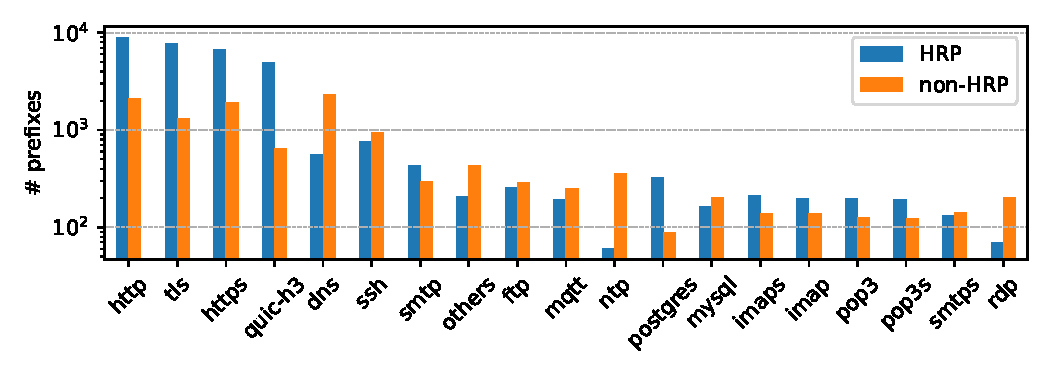
\includegraphics[width=\columnwidth]{./data/plots/services_prefix_tls_others.pdf}
\caption{Services identified on anycast prefixes.}
\vspace*{-4mm}
\label{fig:services_prefix}
\end{figure}

We analyze the detected open ports and their underlying protocols to evaluate how strictly anycast networks adhere to IANA port assignments~\cite{iana-port-service}.
Across all measured ports, 84\% of identified services run the expected protocol. Excluding the highly prevalent TLS and HTTP services increases adherence to 94\%.
As in prior work~\cite{lzr}, we observe that port 80 responds to HTTP in 93\% of cases.
Services on anycast prefixes are likely commercial and user-facing, leading to the high port-protocol adherence we observe.

\vspace{0.2em}\noindent\textbf{Web} --
We find that the majority of anycast is used to replicate web servers (running HTTP/HTTP(s) or HTTP/3 with QUIC).
In total, 86\% %(11k)
of /24s prefixes, and 56\% (553) of ASes have a web service hosted, while 42\% %(5k)
prefixes and 16\% (165) of ASes have HTTP/3 services.
We find that web services are also hosted on ports 8080 and 8443 (22\%) and on other non-standard ports (15\%), in addition to the common ports (80 and 443).
While prior work~\cite{SattlerEtAl_PackedBrimInvestigating_2023} observed a high prevalence of web services on \gls{hrp}, this trend also extends to anycast deployments.
Web content can benefit from replication using anycast~\cite{_CloudflareCache_2026, moura-anycast-ddos}.
For instance, Cloudflare functions as a reverse proxy, caching content across various geographic locations to ensure proximity to the user~\cite{cloudflare-dns}.

\vspace{0.2em}\noindent\textbf{DNS} --
We observe that DNS is largely deployed via anycast on 22\% (\num{2.9e3}) of prefixes, covering 61\% (658) ASes, with most DNS servers on non-\glspl{hrp} (80\%).
The top DNS providers include Amazon (15\% of /24-prefixes), Identity Digital (7\%), Cloudflare (3\%), NetActuate (3\%), and Vercara (3\%), which are big DNS providers.
We find DNS over QUIC (UDP/853) deployments in small numbers (\num{1338} IPs), where 95\% of the IP addresses originate from NextDNS (AS34939).
By querying \texttt{CHAOS TXT} records from multiple \glspl{vp}, we find 25 ASes (including root server and \gls{cctld} operators) run different DNS software across \glspl{pop} sharing the same anycast address (detailed in Appendix~\ref{app:dns-software}).

To investigate the dependency of DNS on anycast, we look at registered domain names under well over 1000 legacy and new \glspl{gtld} 
using \openintel data~\cite{openintel}.
The \dataset is from February 18th, 2026, with \num{204.1e6} domains.
We label domain names as using anycast based on whether all the domain's authoritative name server A records match anycast prefixes in our \dataset, unicast if none match, or a mix of both.
We find that 72\% of domains rely on at least one anycast authoritative name server, while 4\% rely on a mix of anycast and unicast authoritative name servers.
Mix deployments can result in higher DNS name resolution latency~\cite{moritz-recursive}.
Sommese \etal studied anycast adoption in authoritative DNS in 2021.
We see that anycast adoption grew (57\% in 2021) and mix deployments decreased (5\% in 2021).
Our \dataset includes 43\% more /24 anycast prefixes than in 2021, which may contribute to the observed growth.
In the Sommese \etal study, they aggregate \glspl{cctld} in their analysis, but these are closed data and difficult to obtain.
We argue that \glspl{gtld} provide a generic yet comprehensive view of global trends in DNS, given their size in terms of domain names.
We look at the effect of adding open \glspl{cctld} (\eg, \texttt{.ch} and \texttt{.se}, \num{3.7e6} domain names) and we find marginal changes ($<$1\%).

To find the distribution of domains using exclusively anycast infrastructure, we observe that 28\% of domain names in our \gls{gtld} \dataset rely on Host Europe, 22\% on Cloudflare, 8\% on Google, 5\% on Vercara, and 3\% on IONOS.
Hence, a significant portion of domain names from \glspl{gtld} rely on a few anycast DNS providers.

\vspace{0.2em}\noindent\textbf{SSH}\label{subsec:ssh} --
Surprisingly, we see SSH servers in anycast prefixes: 13\% (\num{1.7e3}) of prefixes across 20\% (215) ASes.
SSH is typically used for remote management, where service replication across anycast nodes is counterintuitive.
To determine whether our \glspl{vp} reaches the same physical machine, we conducted an additional ZGrab2 scan on March 5th, 2026, collecting SSH host keys.
However, if system administrators reuse the same host key when creating a new anycast node, different machines may end up with identical keys.
We find in 70 cases where the \gls{vp} see a different key, suggesting different machines.
Furthermore, this practice suggests that clients may connect to different SSH servers based on their location (the nearest node), as we suspect SSH is not replicated.
Operationally, SSH should use unicast addresses of the machine on which it is configured.
However, if misconfigured, SSH may be unintentionally exposed to anycast address due to the OpenSSH daemon, which listens on all local addresses by default~\cite{_Sshd_config5OpenBSDManual_}.
% https://man.openbsd.org/sshd_config#ListenAddress
% https://www.cyberciti.biz/tips/howto-openssh-sshd-listen-multiple-ip-address.html

\vspace{0.2em}\noindent\textbf{Mail} --
We detect IMAP(s) or POP3(s) on 376 (3\%) anycast prefixes and SMTP(s) on 746 (6\%).
Mail infrastructure is consolidated, with just five providers--Nazwa.pl, Amazon, Google, OVH, and Fly.io--accounting for 70\% of the identified mail services.
Since POP3 and IMAP are used to store and retrieve email, we cannot determine whether the deployments are fully replicated backend mail or they function as edge proxies~\cite{Khalidi_HowMicrosoftBuilds_2017} distributed across multiple locations.
We find \num{2346} anycast IP addresses hosting SMTPS on port 465, which is used for secure mail communication between clients and mail servers (submission)~\cite{rfc8314}.
We inspect the TLS certificates of these servers to understand what type of email servers they are.
We observe a long tail distribution, where 46\% IPs have certificates with \textit{smtp.gmail.com} as subject name, under Google's infrastructure (AS15169), where the certificates are issued by Google Trust Services WR4~\cite{_GoogleTrustServices_}, and valid for 90 days, suggesting \textit{Gmail} instances. 
Following, 6\% have certificates with \textit{netart.com} as subject name, under Nazwa.pl (AS15967), where the certificate is issued by \textit{netartSSL}.

\vspace{0.2em}\noindent\textbf{Other notable services} --
We observe a few instances of \gls{ntp} servers.
3\% of prefixes (420) are spread across 13\% of ASes (144), with the majority being deployed in non-\gls{hrp} (360 cases). In total, we find \num{1951} IP addresses hosting \gls{ntp}\@.
While \gls{ntp} can be deployed using anycast, operational challenges exist~\cite{rfc8633}, including time inconsistencies caused by routing changes, the inability for clients to distinguish between servers sharing the same anycast address, and the need for multiple independent server addresses despite anycast deployment.
%First, rapid changes in the anycast topology may cause incoherence in the time that clients receive, as the client has no way of distinguishing between the different \glspl{pop}.
%Second, the closest routed server may be faulty, but clients cannot switch to another one if they are sharing the same IP address using anycast.
%Third, configuring multiple time servers with an anycast IP address does not exempt from the necessity of providing multiple IP addresses that the client can evaluate and choose among.

Surprisingly, we also detect
database services such as MySQL, PostgreSQL, Redis, MsSQL, MongoDB, and OracleDB on anycast prefixes.
We find in 5\% (726) of the prefixes and 5\% (54) of the ASes.
86\% of the anycast prefixes are from Nazwa.pl, Amazon, Google, OVH, or Fly.io.
Deploying databases over anycast is generally discouraged, as these services rely on long-lived connections that are susceptible to disruption from anycast routing changes~\cite{rfc4786}.
% see rfc4786 section 4.1
We suspect that these servers are in a single location where the anycast \dataset measurements reach their different endpoints.
Furthermore, we suspect that the exposure of databases to the Internet stems from broad interface binding configurations.
For instance, binding MySQL to \texttt{0.0.0.0}~\cite{_MySQLMySQLRouter_} or using the \texttt{*} wildcard in PostgreSQL~\cite{_193ConnectionsAuthentication_2026} causes the daemon to listen on all available local addresses.
However, these are not default configurations, and online tutorials incorrectly recommend them, allowing their users to remotely access the database~\cite{_HowAllowRemote_}.

\subsection{Services, Operators and Resilience}
We investigate the leading operators hosting services on anycast prefixes.
As shown in~\cref{fig:as-service}, Google and Cloudflare are the top ASes hosting the highest volume of services driven by web traffic.
Alongside Identity Digital, 
Amazon hosts the largest share of DNS services.
As a major domain registry and registrar, Identity Digital relies on anycast to provide authoritative DNS for the top-level domains it manages.
Furthermore, we observe that Cloudflare, Google, and Fastly dominate the web services detected on anycast, since they operate large \gls{cdn} and edge computing platforms that heavily rely on anycast to replicate content across their global infrastructure.

\begin{figure}[tb]
\centering
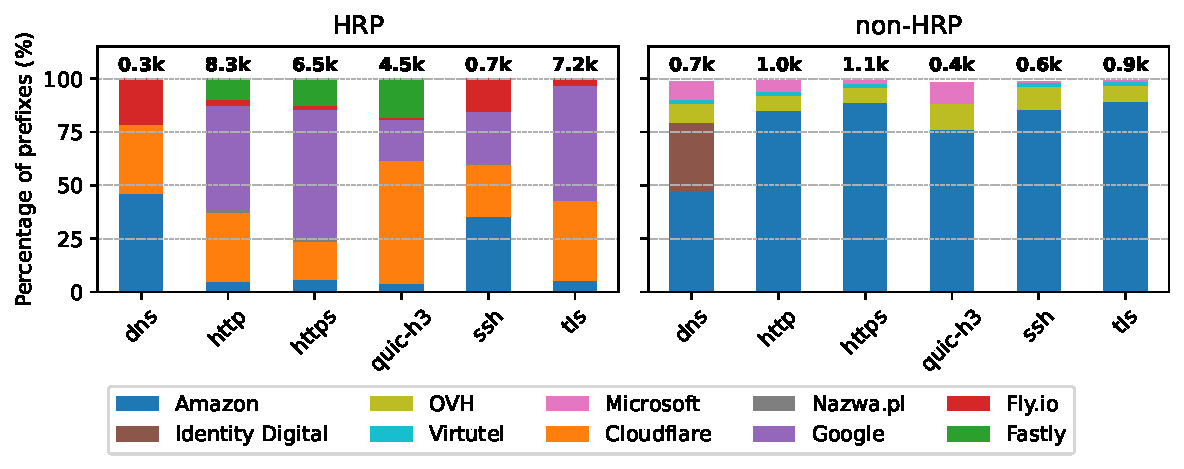
\includegraphics[width=\columnwidth]{./data/plots/providers_services.pdf}
\caption{Top services for the top ASes.}
\vspace*{-4mm}
\label{fig:as-service}
\end{figure}

We find that 52\% (\num{1.5e3}) of the prefixes exclusively host DNS, outnumbering other single-service deployments.
Anycast prefixes can be utilized such that one IP address associated with a service is covered by one advertised prefix (single service on the prefix) or alternatively multiple services are covered by the same prefix~\cite{rfc4786}. % see rfc4786 section 4.4.1 and 4.8
Operationally, hosting multiple services in the same anycast prefix offers advantages in resource utilization and scalability, whereas hosting a single service is used for a small number of critical infrastructure services~\cite{rfc4786}. % see rfc4786 section 4.8.1
Single-service prefixes' isolation strategy helps for DDoS mitigation, as it enables operators to drop malicious traffic at the network edge, for instance, via BGP blackholing~\cite{rfc7999}, without causing latency effects on unrelated services, as clients would be routed to another less optimal \gls{pop}.
% see rfc7999 section 3.1

~\cref{fig:service_pops} correlates our identified services with the number of anycast prefix \glspl{pop}.
Our result suggests a deployment characteristic for anycast, where services are deployed according to a trimodal distribution.
The first cluster of services replicated on less than 15 \glspl{pop}, the second cluster of services replicated on between 15 and 50 \glspl{pop}, and the third cluster of services replicated on more than 50 \glspl{pop}.
We observe that web services on anycast are predominantly hosted on hypergiant infrastructure (\eg, Cloudflare, which has 60+ \glspl{pop} detected in \laces \dataset), where anycast \glspl{hrp} are prevalent.
Conversely, non-\gls{hrp} anycast deployments typically operate on a smaller scale, with the majority of the 779 ASes maintaining fewer than 15 \glspl{pop}.
A notable exception is Amazon, which accounts for 88\% of non-\gls{hrp} prefixes exceeding 50 \glspl{pop}.
For DNS, deployments are concentrated on non-\gls{hrp} prefixes (\num{1.5e3}, 65\%) and replicated across different numbers of \glspl{pop}.
The results show that anycast deployments follow three distinct scales, indicating that operators adopt different strategies for the service.
Web services are replicated mainly on large-scale infrastructure and DNS at different scales.
Anycast services inherently benefit from distributed \glspl{pop}, where if one \gls{pop} becomes unavailable, traffic is seamlessly routed to the next (often the closest) location, enhancing service resilience. 

We analyze services in \num{1211} prefixes anycasted within a single continent to evaluate the regional deployment patterns.
North America hosts the most DNS overall (21\%), followed by Europe (10\%), and has a presence in all continents.
However, web services lead the anycast deployment across the board.
QUIC is present in high numbers in North America (19\%), but surprisingly not much in Europe (1\%) or Asia (2\%).
Overall, these results suggest that regional anycast deployments are primarily used to support web services, and that Europe lags behind in local modern web service provision (\eg, QUIC). 
DNS infrastructure is in smaller numbers across the regions.
However, initiatives to regionalize DNS have been taken.
For example, \textit{DNS4EU} replicates DNS resolvers within Europe~\cite{dns4eu_public}.
With current geopolitical discussions regarding data sovereignty~\cite{eu-sovereign}, we may see more operators deploy regional anycast within their jurisdiction.

\begin{figure}[tb]
\centering
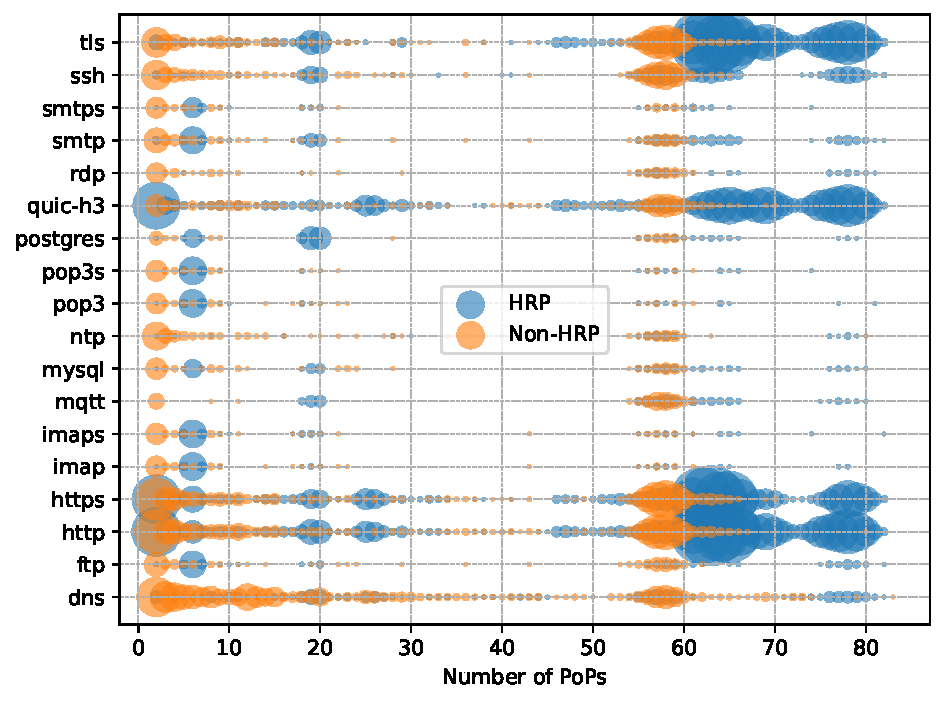
\includegraphics[width=\columnwidth]{./data/plots/service_pops_filtered.pdf}
\caption{Distribution of number of \glspl{pop} for each service.}
\vspace*{-4mm}
\label{fig:service_pops}
\end{figure}

\subsection{Distributed Port Scanning}
\label{subsec:distributed-port-scanning}
To understand how service visibility varies by location, we compare the services detected on anycast prefixes from our European and Oceanian \glspl{vp} using a snapshot of February 18th, 2026.
We find that 4\% (560) of the prefixes classified as \glspl{hrp} from Oceania are entirely unresponsive to TCP or UDP probes from Europe.
Within this unresponsive subset, we detect services on only 44 distinct prefixes ($<$1\% of all anycast prefixes), the majority of which are DNS (37\%, 24 prefixes).
Furthermore, roughly 30\% (\num{4e3}) of the prefixes classified as anycast \glspl{hrp} from Oceania do respond to TCP and UDP probes from Europe, yet fail to meet the \gls{hrp} criteria from the European \gls{vp}.
We observe that 80\% of such prefixes have 151 or fewer TCP-responsive IP addresses, indicating that the entire prefix is not blocked, but rather that a portion of the IP addresses are not served to the European \gls{vp}.

To quantify overall measurement consistency, we calculate the Jaccard similarity index--the intersection of prefixes of a given detected service over their union--across the different \glspl{vp}.
We observe an average similarity of 0.8, indicating that services are mostly deployed on the same prefixes regardless of the observer's location.
We suspect that discrepancies in service visibility are primarily attributable to unpredictable, transient network issues, as found in prior work~\cite{wan-origin-scanning}.

We validate our findings with a follow-up measurement on March 3rd, 2026, by adding a third \gls{vp} in Europe.
Results are consistent with the February 18th measurement, in which the third \gls{vp} and the \gls{vp} in Oceania show a Jaccard index of 0.9, with HTTP mostly affected.
However, we still observe a high dominance of web services on anycast, and hence, this measurement artifact does not change our overall conclusions.
